% Send to Mandar,Jayesh,Arnab,Deepak and perhaps Rahee, PEB, AAO, Michael Richards, John W, Jaydeep K, and Grace Gu, GR Gogate, Chaitanya Bapat, Shekhar Divekar, Hrishikesh, Shilpa, maybe Prem Andrade, Aaron Ashwin
\documentclass[12pt]{article}
\usepackage{amsmath}
\usepackage{amsfonts}
\usepackage{cite}
\usepackage{url}
\usepackage{graphicx}
\usepackage{subcaption}
\usepackage{multirow}
\usepackage{draftwatermark}
\usepackage{pgffor}
% usually hyperref has to be the last package imported
\usepackage{hyperref}
\SetWatermarkText{Draft}
\SetWatermarkScale{5}
%
\newcommand{\beq}{\begin{equation}}
\newcommand{\eeq}{\end{equation}}
\newcommand{\ber}{\begin{eqnarray}}
\newcommand{\eer}{\end{eqnarray}}
\newcommand{\nn}{\nonumber}
\newcommand{\dd}[2]{\frac{d}{d{#2}}{(#1)} }
\newcommand{\pdd}[2]{\frac{\partial}{\partial{#2}}{(#1)} }
% define variables for \mupics command
\newcommand{\nhgscalefactor}{0.2}
\newcommand{\nhgfigheight}{4.0cm}

\def\nhgvala{true}
\def\nhgvalb{exxeyy}
\def\nhgvalc{exxeyynoise}
\def\nhgvald{eyy}
\def\nhgvale{eyynoise}
\def\nhgvalf{uxuy}
\def\nhgvalg{uy}
\def\nhgvalh{uynoise}
\newcommand{\nhgcapmap}[1]{
% https://tex.stackexchange.com/questions/584836/if-statements-in-latex?noredirect=1#comment1470068_584836  
  \edef\temparg{#1}
  \ifx\temparg\nhgvala  True  \fi
  \ifx\temparg\nhgvalb  $\epsilon_{xx}$ \& $\epsilon_{yy}$  \fi
  \ifx\temparg\nhgvalc  (b) + noise \fi
  \ifx\temparg\nhgvald  $\epsilon_{yy}$ \fi
  \ifx\temparg\nhgvale  $\epsilon_{yy}$ + noise\fi
  \ifx\temparg\nhgvalf  $u_x+u_y$ \fi
  \ifx\temparg\nhgvalg  $u_y$ \fi
  \ifx\temparg\nhgvalh  $u_y$ + noise\fi
}
%
\newcommand{\nhghfill}[1]{
  \edef\temparg{#1}
  \ifx\temparg\nhgvala\hfill\fi
  \ifx\temparg\nhgvalb\hfill\fi
  \ifx\temparg\nhgvalc\hfill\fi
  \ifx\temparg\nhgvald\fi
  \ifx\temparg\nhgvale\hfill\fi
  \ifx\temparg\nhgvalf\hfill\fi
  \ifx\temparg\nhgvalg\hfill\fi
  \ifx\temparg\nhgvalh\fi
}
\newcommand{\nhgmupics}[1]{
  \foreach \myvar in {\nhgvala,\nhgvalb,\nhgvalc,\nhgvald,\nhgvale,\nhgvalf,\nhgvalg,\nhgvalh}{
    \begin{subfigure}[b]{\nhgscalefactor\linewidth}
      \includegraphics[totalheight=\nhgfigheight]{Figures/final/ex#1/mu\myvar.png}
      \caption{\nhgcapmap{\myvar}}
    \end{subfigure}
    \nhghfill{\myvar}
  }
}
%
\newcommand{\mupics}[1]{
  % 1
  \begin{subfigure}[b]{\nhgscalefactor\linewidth}
    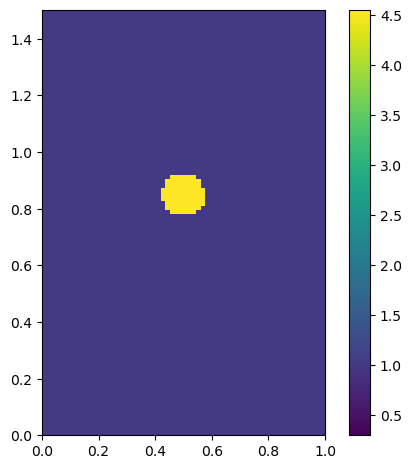
\includegraphics[totalheight=\nhgfigheight]{Figures/final/ex#1/mutrue.png}
    \caption{True}
  \end{subfigure}
  \hfill
  % 2
  \begin{subfigure}[b]{\nhgscalefactor\linewidth}
    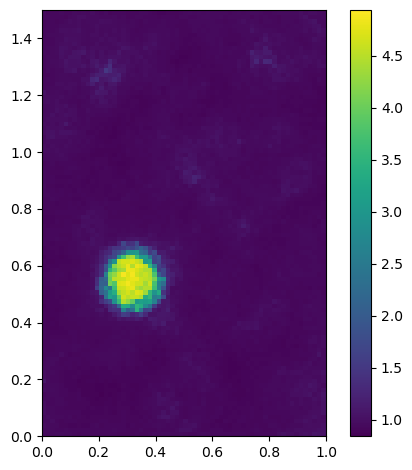
\includegraphics[totalheight=\nhgfigheight]{Figures/final/ex#1/muexxeyy.png}
    \caption{$\epsilon_{xx}$ \& $\epsilon_{yy}$}
  \end{subfigure}
  \hfill
  % 3
  \begin{subfigure}[b]{\nhgscalefactor\linewidth}
    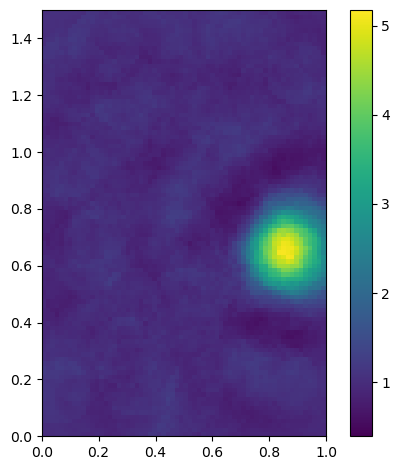
\includegraphics[totalheight=\nhgfigheight]{Figures/final/ex#1/muexxeyynoise.png}
    \caption{(b)+noise}
  \end{subfigure}
  \hfill
  % 4
  \begin{subfigure}[b]{\nhgscalefactor\linewidth}
    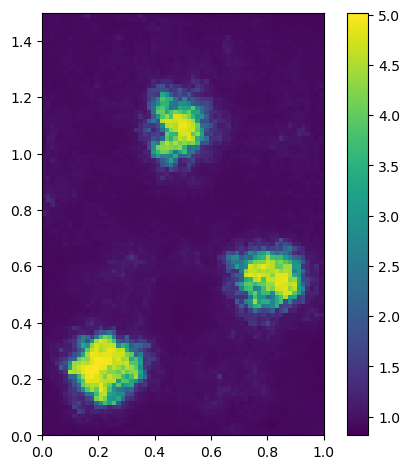
\includegraphics[totalheight=\nhgfigheight]{Figures/final/ex#1/mueyy.png}
    \caption{$\epsilon_{yy}$}
  \end{subfigure}
  % 5
  \begin{subfigure}[b]{\nhgscalefactor\linewidth}
    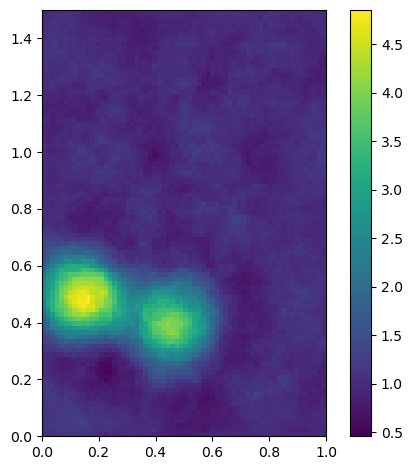
\includegraphics[totalheight=\nhgfigheight]{Figures/final/ex#1/mueyynoise.png}
    \caption{$\epsilon_{yy}$ + noise}
  \end{subfigure}
  \hfill
  % 6
  \begin{subfigure}[b]{\nhgscalefactor\linewidth}
    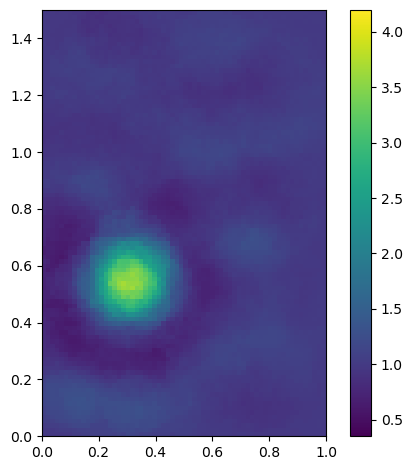
\includegraphics[totalheight=\nhgfigheight]{Figures/final/ex#1/muuxuy.png}
    \caption{$u_{x}$ \& $u_y$}
  \end{subfigure}
  \hfill
  % 7
  \begin{subfigure}[b]{\nhgscalefactor\linewidth}
    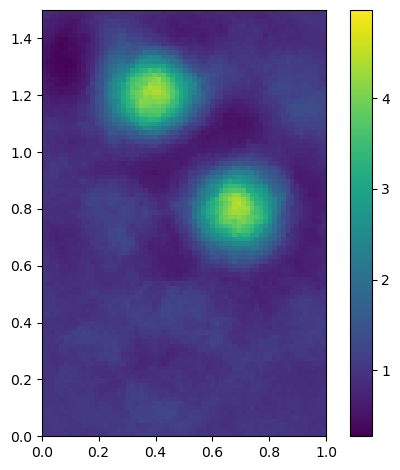
\includegraphics[totalheight=\nhgfigheight]{Figures/final/ex#1/muuy.png}
    \caption{$u_y$}
  \end{subfigure}
  \hfill
  % 8
  \begin{subfigure}[b]{\nhgscalefactor\linewidth}
    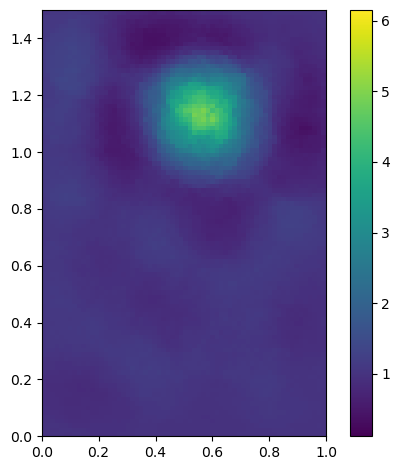
\includegraphics[totalheight=\nhgfigheight]{Figures/final/ex#1/muuynoise.png}
    \caption{$u_y$+noise}
  \end{subfigure}
}



\begin{document}
% bib
\title{Elasticity imaging using a Convolutional Neural Network}
\author{Nachiket Gokhale\footnote{The author is very grateful to Paul Barbone (Professor, Mechanical Engineering, Boston University, Boston MA, USA.) for patiently answering many questions about finite elements. Conversations with Arnab Majumdar (ArcVisions, Kolkata, India), Michael Richards ( University of Rochester, NY, USA) and Mandar Kulkarni (CGG Veritas, Houston, TX, USA) are gratefully acknowledged and appreciated.}\\gokhalen@gmail.com}
\date{\today}
\maketitle
\abstract{We explore the application of a Convolutional Neural Network (CNN) using labeled data (supervised learning) to image the shear modulus field of an almost incompressible elastic medium in plane strain using displacement or strain field data. This problem is important in medicine because the shear modulus of suspicious and potentially cancerous growths in soft tissue is elevated by about an order of magnitude as compared to the background of normal tissue. Therefore, imaging the stiffness leads to high-contrast medical images. Our prediction problem is as follows: \textit{Given displacement or strain fields, predict the shear modulus field}. Our CNN is trained using 2400 training examples consist of displacement or strain fields and a corresponding shear modulus field. We present encouraging results which warrant further research and show the promise of this methodology.}
\section{Introduction}
The shear modulus of palpable nodules (which can be thought of as abnormal and potentially cancerous growths in soft tissue) is approximately an order of magnitude higher than the stiffness of the background of normal glandular tissue \cite{paper:sarv1998}. See also Figure (\ref{fig:shearmod}). It follows then, that imaging the shear modulus of soft tissue results in a high-contrast imaging method because suspicious growths will stand out clearly against the background of normal tissue. Elasticity Imaging is a broad term that refers to methods which image the shear modulus (or other elastic properties) of soft tissue in various ways. See \cite{paper:gao1996,paper:parker2010,book:alamgarra2019,bookchap:oberaibarbone2019} for a comprehensive reviews of the field.
%
\begin{figure}
   \centering
    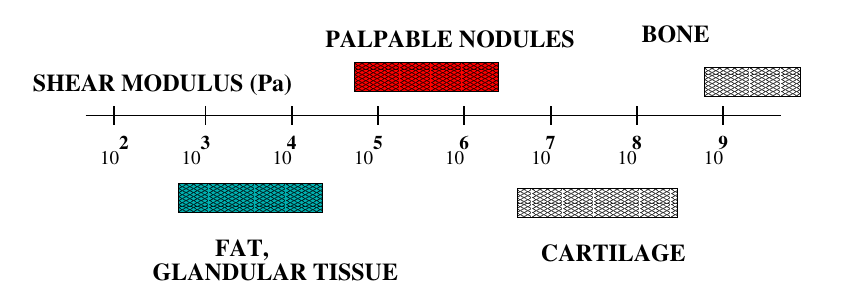
\includegraphics[totalheight=3cm]{Figures/shearmod.png}
  \caption{\label{fig:shearmod} Shear moduli of different types of soft tissue. Adapted from Figure 1 in \cite{paper:sarv1998}.}
\end{figure}
%
\begin{figure}
   \centering
    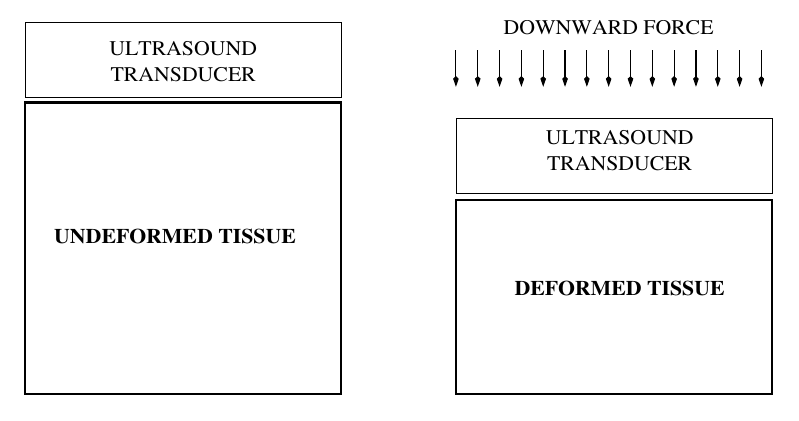
\includegraphics[totalheight=5cm]{Figures/prepostimage.png}
  \caption{\label{fig:prepostimage} Schematic figure showing medical image acquisition when soft tissue is being deformed using ultrasound imaging. The image taken on the left is referred to as the \textit{pre-deformation} image and the image on the right is the \textit{post-deformation image}.}
\end{figure}
%
\subsection{Steps involved in elasticity imaging}
Elasticity Imaging typically consists of  the steps of image acquisition, image registration, and inverse problem solution. These steps are discussed in the following sections.
\subsubsection{Image acquisition} Images of soft tissue undergoing deformation are acquired using various imaging modalities such as ultrasound or magnetic resonance imaging. While time dependent images can be acquired, we shall consider here only two images: a \textit{pre-deformation image} acquired before force is applied and a \textit{post-deformation image} acquired after force is applied. This process is shown in Figure (\ref{fig:prepostimage}) for ultrasound imaging. Also see Figure 2 in \cite{paper:konofagou2004}.
\subsubsection{Image registration} The goal in this step is to find a map between the pre-deformation image and the post-deformation image. For every point in the pre-deformation image we aim to find its location in the post-deformation image. This gives us the \textit{displacement field} between the two images. This displacement field is often referred to as the \textit{measured displacement field}. See \cite{paper:richards2009,paper:gokhale2004,paper:pellot-barakat2004} for minimization based approaches for computing the displacement field. See \cite{paper:ophir1991,paper:ophir1996,paper:alam1998} and references therein for cross-correlation based approaches.
\subsubsection{Inverse problem solution:} The goal in this step is to infer the spatial distribution of the shear modulus from the displacement field. This is called an \textit{inverse problem} because the typical boundary value problem in linear elasticity (referred to as the \textit{forward problem}) is to determine the displacement field given the shear-modulus field. The approaches for inverse problem solution can be divided into two categories: direct and iterative.
\subsubsection{Direct approach} Direct approaches involve solving a single partial differential equation (pde) to obtain the distribution of shear modulus directly: see \cite{paper:raghavan1994,paper:barboneadjwt,paper:albocher}. The coefficients of this pde depend on the measured displacement field. Such approaches are fast and work well when the measured strain field is completely known and has low noise.
\subsubsection{Iterative approach} Iterative approaches \cite{paper:oberai2003,paper:gokhale2008,paper:kalle1996,paper:doyley,paper:goenezen2011} involve guessing a distribution for the shear modulus, solving a linear elasticity forward problem to obtain the predicted displacements, comparing the predicted displacements to the measured displacements and updating the guessed shear modulus distribution using a suitable optimization procedure such as a modified Newton Raphson scheme as in \cite{paper:doyley} or the BFGS scheme as in \cite{paper:gokhale2008,paper:goenezen2011}. Such approaches are typically slower than direct methods, since the require the solution of $\approx$ 25-100 forward problems, but have the ability to handle incomplete data and complex material models.
\subsubsection{Solving the inverse problem with CNNs}
We believe that solving the inverse problem with CNNs can combine the best characteristics of the direct and iterative approaches. The CNN based approach can yield a quick answer, can accomodate complex constitutive relations, can work with incomplete data (e.g. only a single component of a displacement field) and can work with noisy data.
\section{Neural networks and problem setup}
In recent years, neural networks have been applied to various applications such as image classificaton \cite{paper:hinton2017}, hand written digit recognition \cite{paper:kulkarni2018}, solving differential equations and symbolic integration \cite{misc:lample2019}, solving complex partial differential equations such as the Navier-Stokes equation \cite{misc:anandkumar2020}, self-driving cars \cite{misc:agnihotri2019,misc:nvidiaselfdriving2016}, chaos \cite{paper:pathak2018}, natural language processing \cite{misc:googlenlp} and face recognition \cite{conf:taigman2014}. Several effective Machine Learning frameworks such as Google's TensorFlow \cite{misc:tensorflow}, Facebook's PyTorch \cite{incollect:pytorch}, Scikit-Learn \cite{paper:scikit-learn} are freely available. See \cite{misc:compdeep} for a complete list. The interested reader is referred to \cite{book:aggarwal,book:goodfellow,book:chollet,misc:cs231n,misc:andrewng,misc:udemy} for further information about neural networks.
\subsection{Neural networks and elasticity imaging}
Given the success achieved by neural networks on the wide variety of applications cited, it is natural to explore the application of neural networks to the inverse problem of elasticity imaging and several recent efforts \cite{paper:pateloberai2019,misc:gu2020,paper:hoeriginsana2016} have done so. In \cite{paper:pateloberai2019}, the authors use a convolutional neural network to classify specimens into elastically heterogeneous or elastically nonlinear. In \cite{paper:hoeriginsana2016}, the authors use a neural network to estimate strains and stress and then calculate elastic parameters. In \cite{misc:gu2020}, the authors use a neural network which predicts elasticity distributions using residual force maps to update the weights of the neural network. \\In contrast, in this work we compute the shear modulus field from the displacement or strain field using a CNN. There are no physical constraints involved in our work. It is purely a mapping problem from the space of displacement or strain fields to the space of the shear modulus fields. The input data for our CNN is a set of strain or displacement fields or components thereof. For each input there is a corresponding target shear modulus field. The CNN predicts shear modulus fields compares them with the target fields to compute the loss function and its gradient. Thus the CNN learns weights for its filters and other parameters. Using this learned information the CNN is able to predict a shear modulus field from the input data of strain or displacement fields. See Figure (\ref{fig:schematic_inv}).
%
\begin{figure}
   \centering
    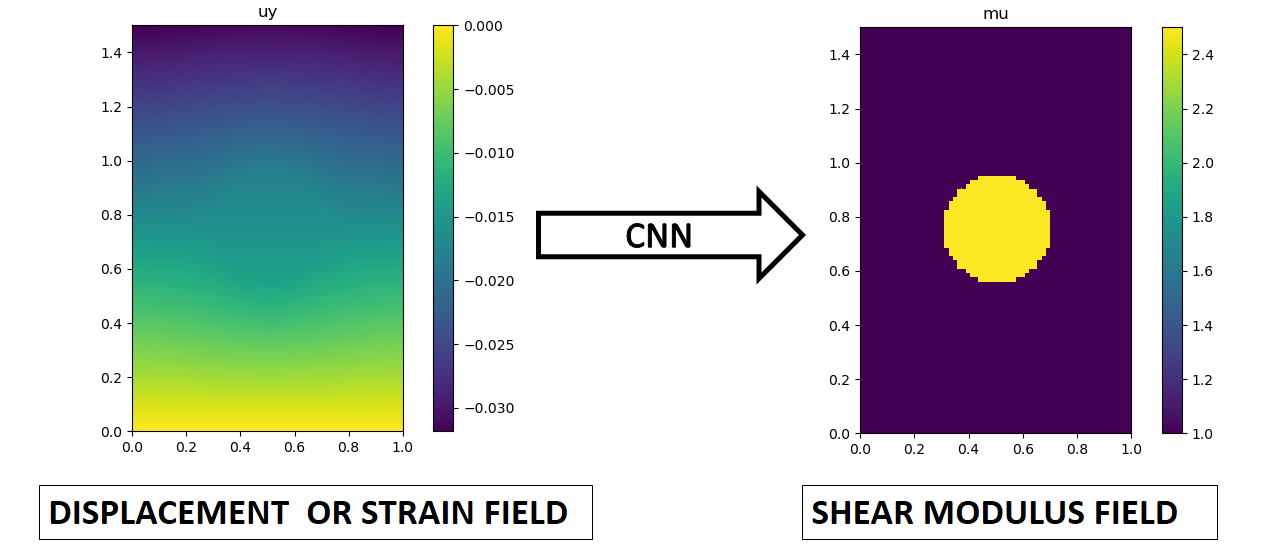
\includegraphics[totalheight=5cm]{Figures/schematic_inv/schematic_inv.png}
  \caption{\label{fig:schematic_inv} Solving the inverse problem using CNNs. The displacement or strain field (or components thereof) are mapped by the CNN into a shear modulus field.}
\end{figure}
%
\subsection{\label{sect:cnnarch} CNN architecture used in this work}
The typical architecture of the CNN we use in this work is shown in Figure (\ref{fig:typical_cnn}) and its parameters are given in Table (\ref{tab:cnnparams}). This CNN was implemented in TensorFlow \cite{misc:tensorflow}. The first dimension '?' represents the number of examples to be processed for training, validation or evaluation. Thus, the first training example is a three dimensional array and can be accessed using the indices $[0,:,:,:]$ (using Numpy notation) and similarly for the others. The second and third dimensions represent the number of nodes in the $y$ and $x$ direction respectively. The last dimension represents the number of channels in the image. In image-processing the number of channels is typically $3$, one channel each for the three colors red, green and blue (RGB). In our case, the number of channels is the number of independent fields in our problem. If we use three independent components of the strain field $\epsilon_{xx},\epsilon_{yy},\epsilon_{xy}$ then the number of channels is $3$. If we use only a single component of the strain field, say $\epsilon_{xx}$ only, then the number of channels is $1$. The \textit{loss function} is \textit{mean squared error} and the optimizer is \textit{Adam}. No regularization is used.  Each CNN has approximately $3.35$ million trainable parameters.
\begin{table}
  \centering
 \begin{tabular}{|c|c|}
   \hline
   CNN Layer & Specifications \\
   \hline
   conv2d    & $32$ filters, kernel size $3$, activation is \textit{relu}, no regularization\\
   \hline
   max\_pooling2d: & pool size $2$, strides $2$\\
   \hline
   conv2d\_1 & $64$ filters, kernel size $3$, activation is \textit{relu}, no regularization\\
   \hline
   max\_pooling2d\_1: & pool size $2$, strides $2$\\
   \hline
   flatten & -\\
   \hline
   dense   & $128$ units, activation \textit{relu}, no regularization\\
   \hline
   dense\_1 & $nnodex*nnodey$ units, activation \textit{softplus}, no regularization\\
   \hline
 \end{tabular}
 \caption{\label{tab:cnnparams} CNN parameters for the network in Figure (\ref{fig:typical_cnn}).}
\end{table}
%
\begin{figure} 
   \centering
    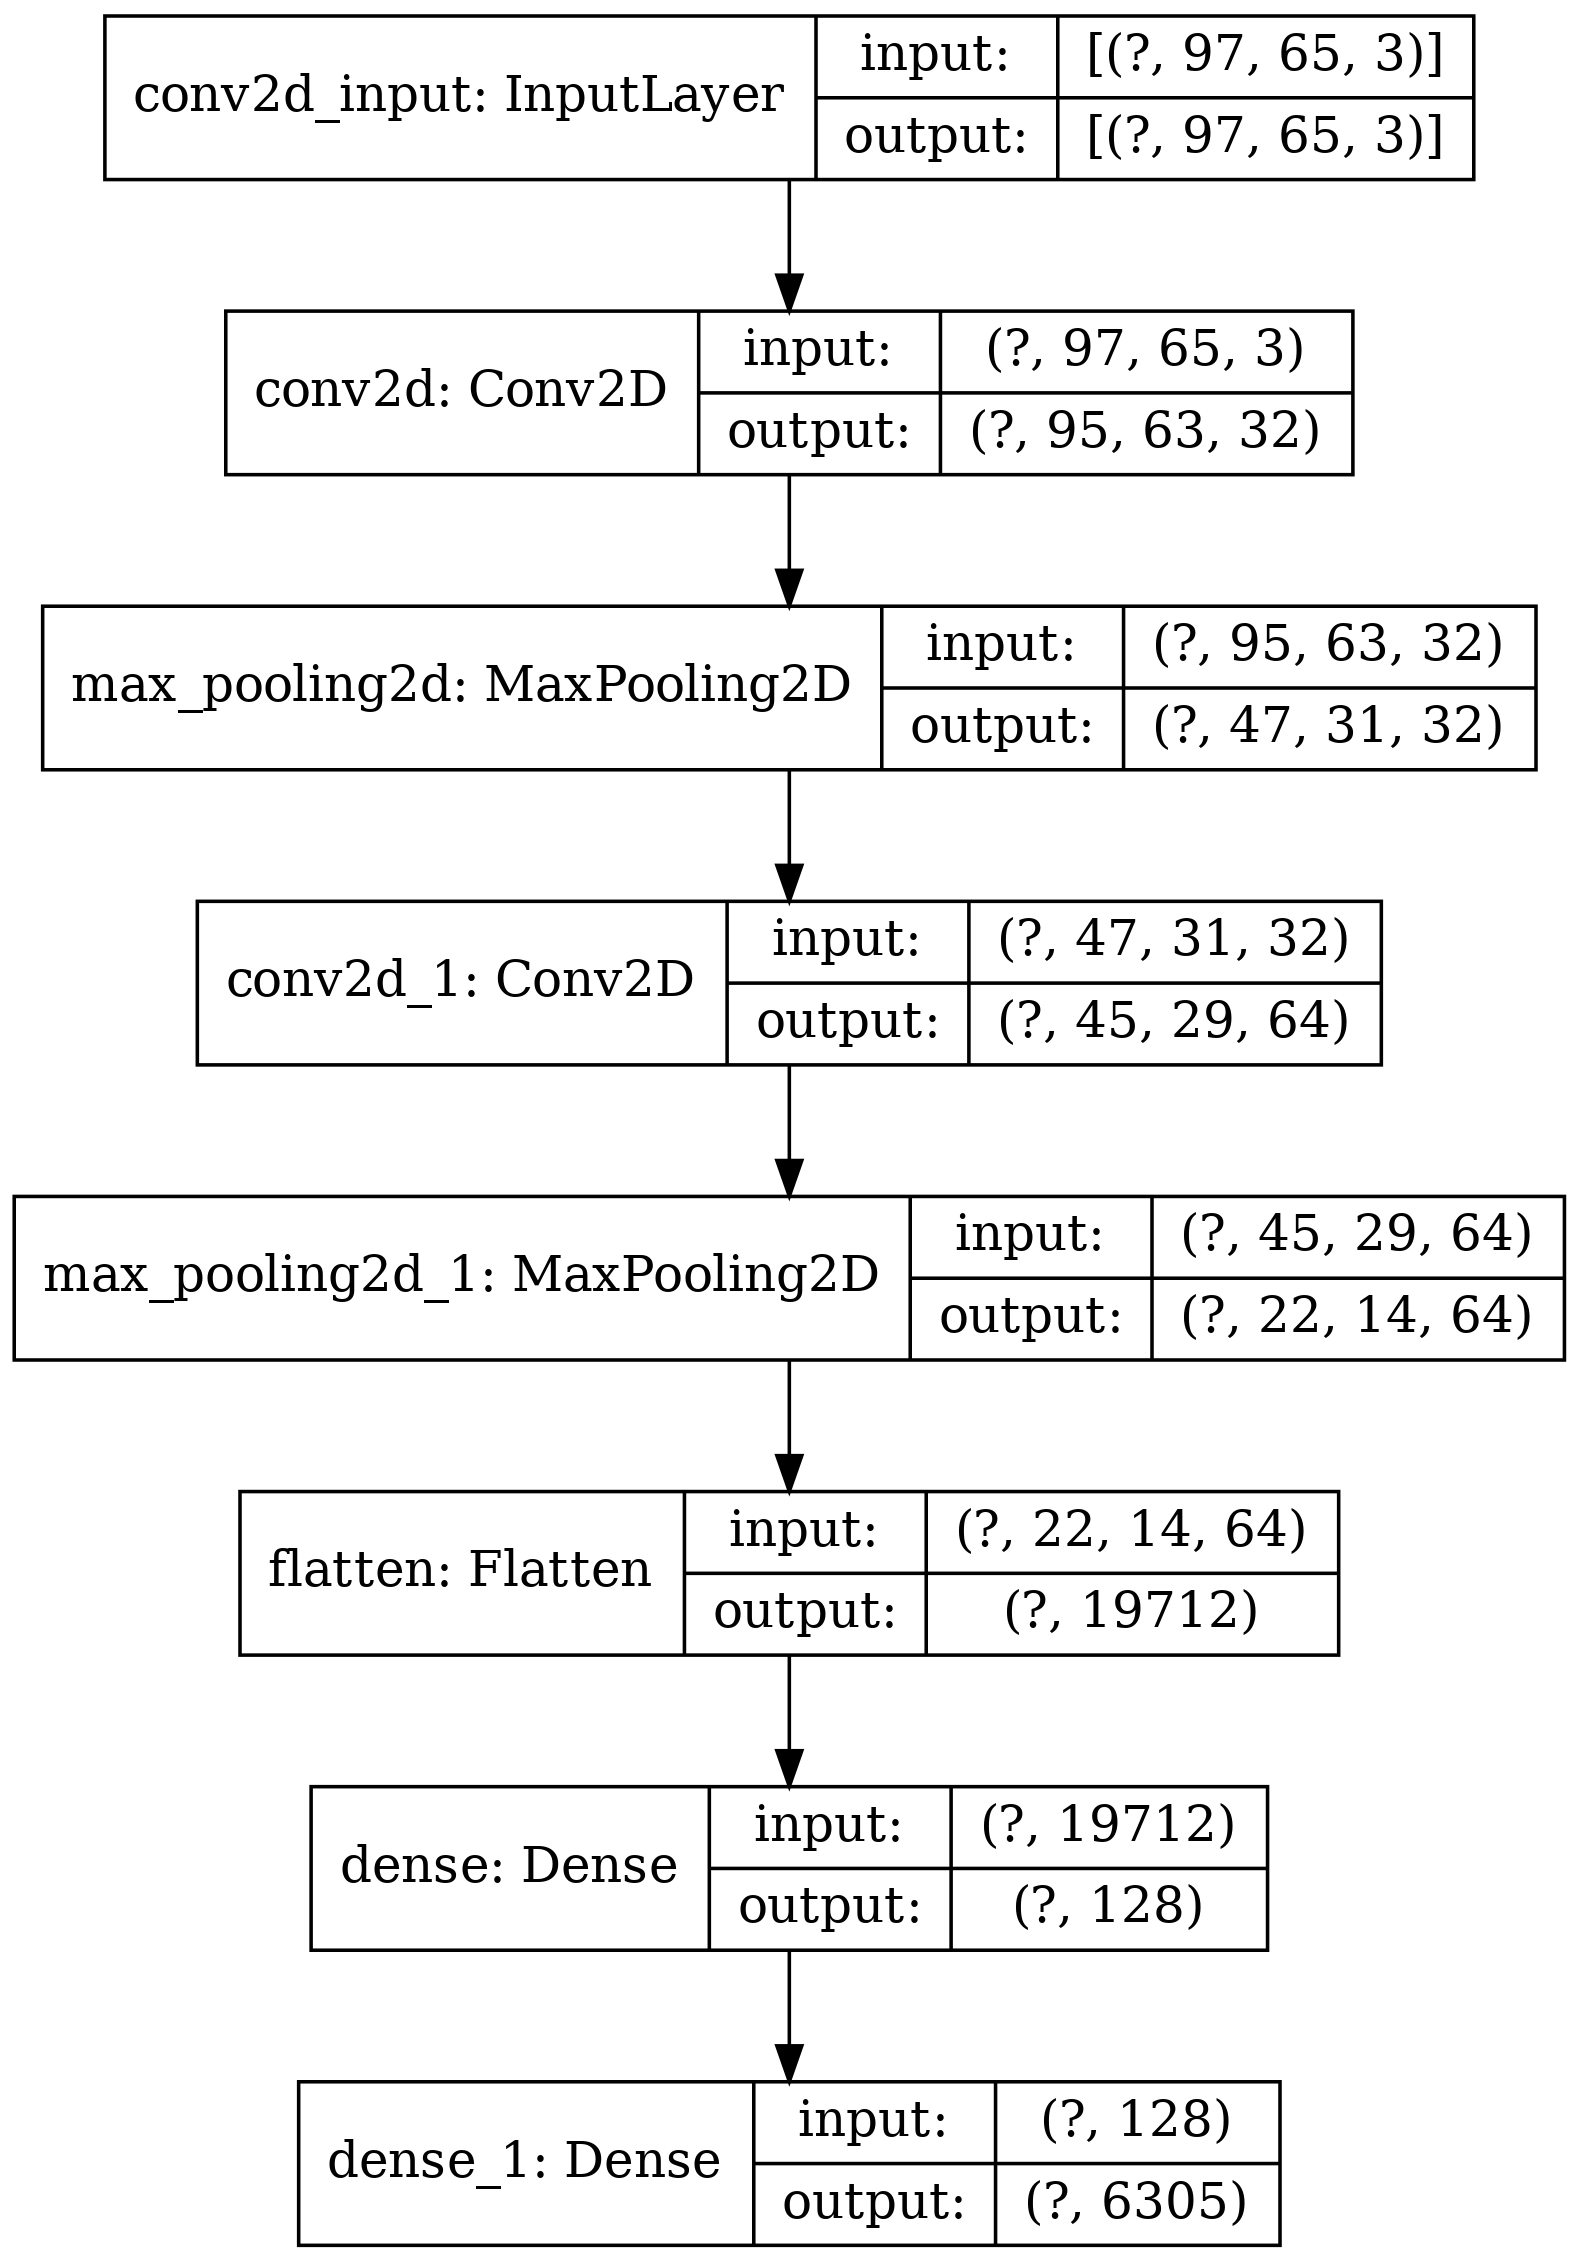
\includegraphics[totalheight=9cm]{Figures/typical_cnn.png}
    \caption{\label{fig:typical_cnn}Typical CNN architecture used in this work. This architecure is essentially the same the one used in the Deep Learning example in \cite{misc:udemy}.}
\end{figure}
%
%
\subsection{\label{sect:probsetup}Problem setup}
The displacement or strain field data required for the CNN is generated using a linear finite element solver named FyPy (\textbf{Fy}nite Elements in \textbf{Py}thon) \cite{misc:fypy}. Both displacements and material properties are interpolated using bilinearly. The problem geometry is shown in Figure (\ref{fig:bc}). The length (in the $x$ direction) is $1.0$ unit. The breadth (in the $y$ direction) is 1.5 units. The background shear modulus is $1.0$ unit. The Poisson's ratio is a constant and is set to $0.49$. There is exactly one inclusion in the domain and its shear modulus is a constant and is a random number ranging from $2.0$ to $5.0$. There are no homogeneous examples. The radius of the inclusion is a random number randing from $0.05$ to $0.15$.\\
$4000$ displacement and strain images are generated and are split into $2400$ training examples, $800$ validation examples and $800$ test examples. When noisy data is used we add noise in the strain or displacement data such that the signal to noise ratio (SNR) is 40dB using equation (\ref{eqn:snr}). The data is made noisy by element wise multiplication of the strain or displacement data with a matrix containing random numbers in the interval $(1-\epsilon,1+\epsilon)$. $\epsilon$ is chosen appropriately to yield $\approx$ 40dB noise. We do not train CNNs with noisy data. Training of the CNN is always carried out on noiseless data and noisy data is given to the CNN as input. 
\begin{equation}
  \label{eqn:snr}
  SNR_{dB} = 20\log_{10}\Big(\frac{\|signal\|_{L^2}}{\|noise\|_{L^2}}\Big)
\end{equation}
The norm $\|\cdot\|_{L^2}$ in the above equation is a discrete $L^2$ norm. 
% Noise details
%
\begin{figure} 
   \centering
    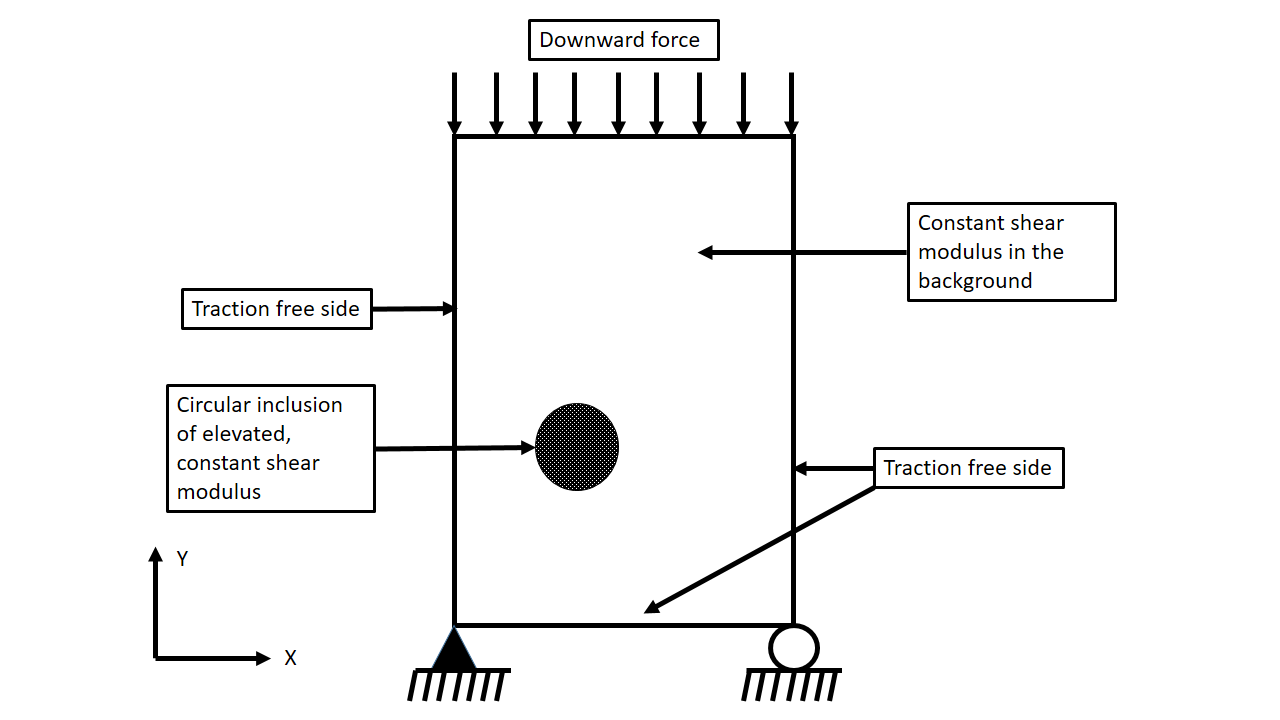
\includegraphics[totalheight=9cm]{Figures/bc.png}
  \caption{\label{fig:bc}Boundary conditions and material properties used in this work. }
\end{figure}
%
\section{Imaging one inclusion}
We apply the CNN described in Section (\ref{sect:cnnarch}) to predict the shear modulus field when only one inclusion is present. The data is generated as described in Section (\ref{sect:probsetup}). As mentioned in Section (\ref{sect:probsetup}), CNNs are trained only on noiseless data and used to make predictions on noisy data. Four CNNs are trained. The training data and prediction data for CNNs is specified in Table (\ref{tab:cnnone:io}). For example, the first entry in Table (\ref{tab:cnnone:io}) should be interpreted as: CNN $\epsilon_{xx}$ \& $\epsilon_{yy}$ is trained on both components of a noiseless strain field (given in column 2) and is used to make predictions using both components of the strain field, with and without noise (given in column 3). The training and loss curves for the CNNs are shown in Figures (\ref{fig:oneinc:trainexxeyy},\ref{fig:oneinc:traineyy},\ref{fig:oneinc:trainuxuy},\ref{fig:oneinc:trainuy}). It is seen that the CNNs trained on strain data show a sharp and early drop in the loss. The CNNs trained on displacement data show slow drop in the loss. The predictions of the various CNNs are shown in Figures (\ref{fig:oneinc:1}-\ref{fig:oneinc:16}). The subcaptions of the figures are explained in Table (\ref{tab:subcap}).\\
The conclusions that can be drawn from Figures (\ref{fig:oneinc:1}-\ref{fig:oneinc:16}) are:
\begin{enumerate}
\item{The location of the inclusion is predicted accurately.}
\item{The shear modulus of small inclusions is under-predicted. See Figures (\ref{fig:oneinc:1},\ref{fig:oneinc:3},\ref{fig:oneinc:6},\ref{fig:oneinc:8}).}
\item{The shear modulus of large inclusions is correct on average. The discontinuities in the true shear modulus field are not predicted accurately. Instead a smooth field is predicted.}
\item{It is observed that a region of high shear modulus has a region of low shear modulus adjoining it. See Figures (\ref{fig:oneinc:1},\ref{fig:oneinc:2},\ref{fig:oneinc:3},\ref{fig:oneinc:3}). }
\end{enumerate}
%
\begin{table}
  \centering
  \begin{tabular}{|l|c|c|}
    \hline
    CNN Name & Training data (noiseless) & Prediction data \\
    \hline
    CNN $\epsilon_{xx}$ \& $\epsilon_{yy}$ & $\epsilon_{xx}$ \& $\epsilon_{yy}$ & $\epsilon_{xx}$ \& $\epsilon_{yy}$ or $\epsilon_{xx}$ \& $\epsilon_{yy}$ + noise\\
    \hline
    CNN $\epsilon_{yy}$ & $\epsilon_{yy}$ & $\epsilon_{yy}$ or $\epsilon_{yy}$ + noise\\
    \hline
    CNN $u_x$ \& $u_y$ & $u_x$ \& $u_y$ & $u_x$ \& $u_y$\\
    \hline
    CNN $u_y$ & $u_y$ & $u_y$ or $u_y$ + noise\\
    \hline
  \end{tabular}
  \caption{\label{tab:cnnone:io} Listing of CNNs trained, their training and prediction data}
\end{table}
%
\begin{table}
  \centering
   \begin{tabular}{cp{8cm}}
    \hline
    \multicolumn{1}{|c|}{Subcaption} & \multicolumn{1}{c|}{Meaning}\\
    \hline
    \multicolumn{1}{|c|}{True} & \multicolumn{1}{p{8cm}|}{This is the true shear modulus field. The input displacement or strain fields correspond to this shear modulus field. This is the ideal prediction of our CNN.}\\
    \hline
    \multicolumn{1}{|c|}{$\epsilon_{xx}$ \& $\epsilon_{yy}$} & \multicolumn{1}{p{8cm}|}{Prediction using CNN $\epsilon_{xx}$ \& $\epsilon_{yy}$ using noiseless $\epsilon_{xx}$ \& $\epsilon_{yy}$}\\
    \hline
    \multicolumn{1}{|c|}{(b) + noise} & \multicolumn{1}{p{8cm}|}{Prediction using CNN $\epsilon_{xx}$ \& $\epsilon_{yy}$ using noisy $\epsilon_{xx}$ \& $\epsilon_{yy}$}\\
    \hline
    \multicolumn{1}{|c|}{$\epsilon_{yy}$} & \multicolumn{1}{p{8cm}|}{Prediction using CNN $\epsilon_{yy}$ using noiseless $\epsilon_{yy}$}\\
    \hline
    \multicolumn{1}{|c|}{$\epsilon_{yy}$ + noise} & \multicolumn{1}{p{8cm}|}{Prediction using CNN $\epsilon_{yy}$ using noisy $\epsilon_{yy}$}\\
    \hline
    \multicolumn{1}{|c|}{$u_x$ \& $u_y$} & \multicolumn{1}{p{8cm}|}{Prediction using CNN $u_x$ \& $u_y$  using noisless $u_x$ \& $u_y$ }\\
    \hline
    \multicolumn{1}{|c|}{$u_y$} & \multicolumn{1}{p{8cm}|}{Prediction using CNN $u_y$  using noisless $u_y$ }\\
    \hline
    \multicolumn{1}{|c|}{$u_y$ + noise} & \multicolumn{1}{p{8cm}|}{Prediction using CNN $u_y$  using noisy $u_y$ }\\
    \hline
  \end{tabular}
  \caption{\label{tab:subcap} Interpretations of subcaptions.}
\end{table}
%
% Training loss, val_loss for exxeyy
\begin{figure}
  %
  \centering
  \begin{subfigure}[b]{0.45\linewidth}
    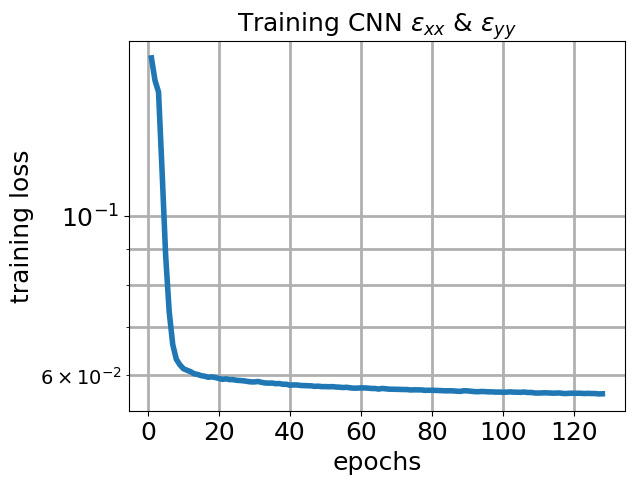
\includegraphics[totalheight=\nhgfigheight]{Figures/final/training/exxeyy/field_strainxxyy_plot_loss.png}
    \caption{Training loss}
  \end{subfigure}
  %
  \begin{subfigure}[b]{0.45\linewidth}
    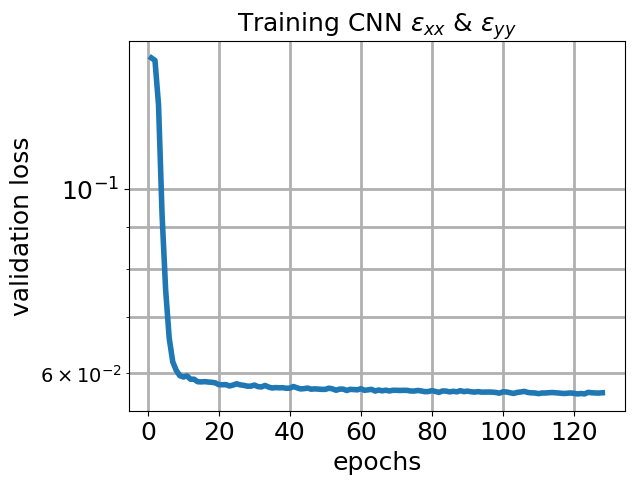
\includegraphics[totalheight=\nhgfigheight]{Figures/final/training/exxeyy/field_strainxxyy_plot_val_loss.png}
    \caption{Validation loss}
  \end{subfigure}
  %
\caption{\label{fig:oneinc:trainexxeyy} Training and validation loss for CNN $\epsilon_{xx}$ \& $\epsilon_{yy}$.}
\end{figure}
% Training loss, val_loss for eyy
\begin{figure}
  %
  \centering
  \begin{subfigure}[b]{0.45\linewidth}
    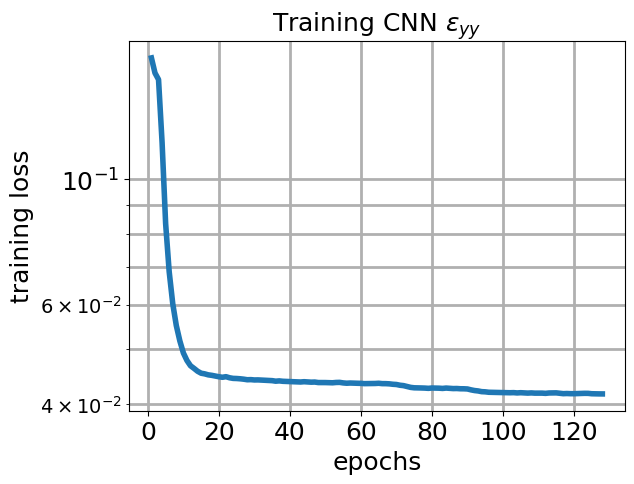
\includegraphics[totalheight=\nhgfigheight]{Figures/final/training/eyy/field_strainyy_plot_loss.png}
    \caption{Training loss}
  \end{subfigure}
  %
  \begin{subfigure}[b]{0.45\linewidth}
    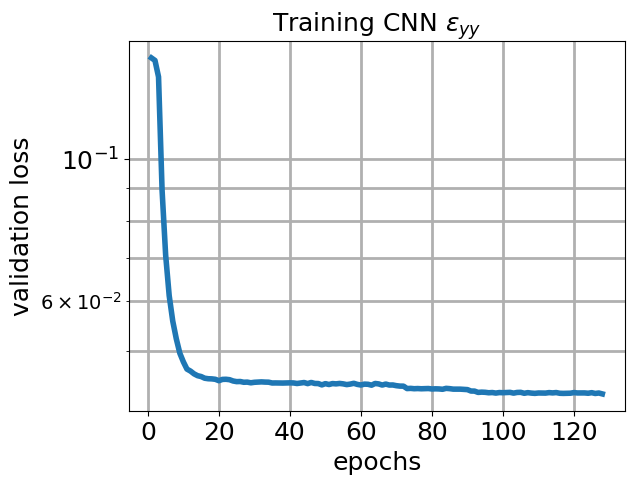
\includegraphics[totalheight=\nhgfigheight]{Figures/final/training/eyy/field_strainyy_plot_val_loss.png}
    \caption{Validation loss}
  \end{subfigure}
  %
\caption{\label{fig:oneinc:traineyy} Training and validation loss for CNN $\epsilon_{yy}$.}
\end{figure} 
% Training loss, val_loss for uxuy
\begin{figure}
  %
  \centering
  \begin{subfigure}[b]{0.45\linewidth}
    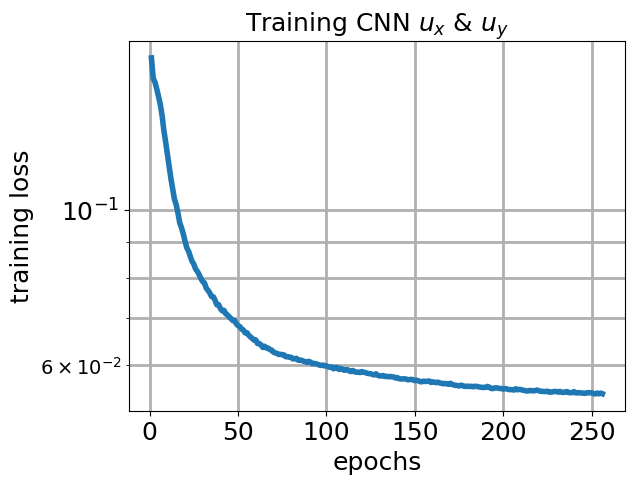
\includegraphics[totalheight=\nhgfigheight]{Figures/final/training/uxuy/field_images_plot_loss.png}
    \caption{Training loss}
  \end{subfigure}
  %
  \begin{subfigure}[b]{0.45\linewidth}
    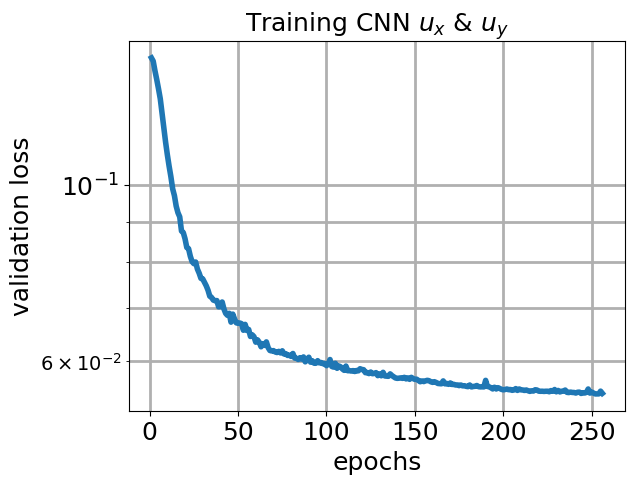
\includegraphics[totalheight=\nhgfigheight]{Figures/final/training/uxuy/field_images_plot_val_loss.png}
    \caption{Validation loss}
  \end{subfigure}
  %
  \caption{\label{fig:oneinc:trainuxuy} Training and validation loss for CNN $u_x$ \& $u_y$.}
\end{figure}
% Training loss, val_loss for uy
\begin{figure}
  %
  \centering
  \begin{subfigure}[b]{0.45\linewidth}
    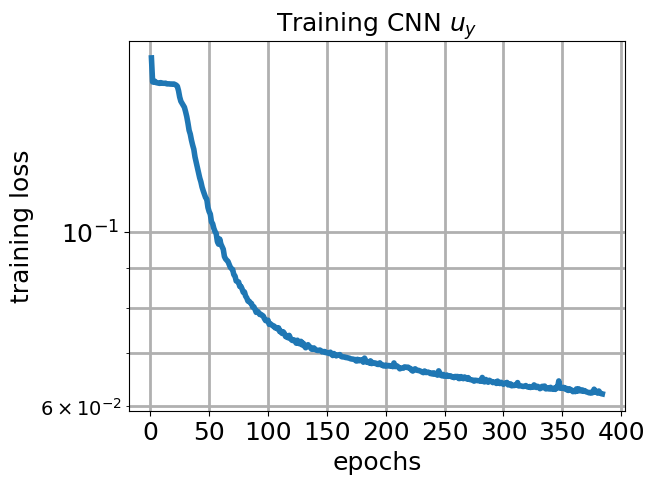
\includegraphics[totalheight=\nhgfigheight]{Figures/final/training/uy/field_imagesy_plot_loss.png}
    \caption{Training loss}
  \end{subfigure}
  %
  \begin{subfigure}[b]{0.45\linewidth}
    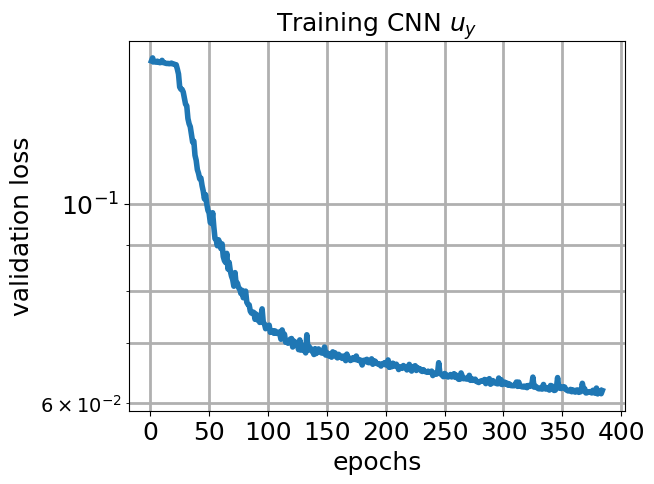
\includegraphics[totalheight=\nhgfigheight]{Figures/final/training/uy/field_imagesy_plot_val_loss.png}
    \caption{Validation loss}
  \end{subfigure}
  %
  \caption{\label{fig:oneinc:trainuy} Training and validation loss for CNN $u_y$.}
\end{figure}
%
% Figure 1
\begin{figure}[h]
  \mupics{1}
  \caption{\label{fig:oneinc:1}Imaging one inclusion: result 1.}
\end{figure}
\newpage
% Figure 2
\begin{figure}[h]
  \mupics{2}
  \caption{\label{fig:oneinc:2}Imaging one inclusion: result 2.}
\end{figure}
\newpage
% Figure 3
\begin{figure}[h]
  \mupics{3}
  \caption{\label{fig:oneinc:3}Imaging one inclusion: result 3.}
\end{figure}
\newpage
% Figure 4
\begin{figure}[h]
  \mupics{4}
  \caption{\label{fig:oneinc:4}Imaging one inclusion: result 4.}
\end{figure}
\newpage
% Figure 5
\begin{figure}[h]
  \mupics{5}
  \caption{\label{fig:oneinc:5}Imaging one inclusion: result 5.}
\end{figure}
\newpage
% Figure 6
\begin{figure}[h]
  \mupics{6}
  \caption{\label{fig:oneinc:6}Imaging one inclusion: result 6.}
\end{figure}
\newpage
% Figure 7
\begin{figure}[h]
  \mupics{7}
  \caption{\label{fig:oneinc:7}Imaging one inclusion: result 7.}
\end{figure}
\newpage
% Figure 8
\begin{figure}[h]
  \mupics{8}
  \caption{\label{fig:oneinc:8}Imaging one inclusion: result 8.}
\end{figure}
\newpage
% Figure 9
\begin{figure}[h]
  \mupics{9}
  \caption{\label{fig:oneinc:9}Imaging one inclusion: result 9.}
\end{figure}
\newpage
% Figure 10
\begin{figure}[h]
  \mupics{10}
  \caption{\label{fig:oneinc:10}Imaging one inclusion: result 10.}
\end{figure}
\newpage
% Figure 11
\begin{figure}[h]
  \mupics{11}
  \caption{\label{fig:oneinc:11}Imaging one inclusion: result 11.}
\end{figure}
\newpage
% Figure 12
\begin{figure}[h]
  \mupics{12}
  \caption{\label{fig:oneinc:12}Imaging one inclusion: result 12.}
\end{figure}
\newpage
% Figure 13
\begin{figure}[h]
  \mupics{13}
  \caption{\label{fig:oneinc:13}Imaging one inclusion: result 13.}
\end{figure}
\newpage
% Figure 14
\begin{figure}[h]
  \mupics{14}
  \caption{\label{fig:oneinc:14}Imaging one inclusion: result 14.}
\end{figure}
\newpage
% Figure 15
\begin{figure}[h]
  \mupics{15}
  \caption{\label{fig:oneinc:15}Imaging one inclusion: result 15.}
\end{figure}
\newpage
% Figure 16
\begin{figure}[h]
  \mupics{16}
  \caption{\label{fig:oneinc:16}Imaging one inclusion: result 16.}
\end{figure}
\newpage
%
% Movies
\begin{table}
  \centering
  \begin{tabular}{|c|c|c|}
    \hline
    Problem data & CNN used & Animation \\
    \hline
    Noiseless $\epsilon_{xx}$ \& $\epsilon_{yy}$ & CNN $\epsilon_{xx}$ \& $\epsilon_{yy}$ & \href{run:movies/one/field\_strainxxyy\_noise\_0.0\_movie.mp4}{Click here}\\
    \hline
    Noisy $\epsilon_{xx}$ \& $\epsilon_{yy}$ & CNN $\epsilon_{xx}$ \& $\epsilon_{yy}$ & \href{run:movies/one/field\_strainxxyy\_noise\_0.02\_movie.mp4}{Click here}\\
    \hline
    Noiseless $\epsilon_{yy}$ & CNN $\epsilon_{yy}$ & \href{run:movies/one/field\_strainyy\_noise\_0.0\_movie.mp4}{Click here}\\
    \hline
    Noisy $\epsilon_{yy}$ & CNN $\epsilon_{yy}$ & \href{run:movies/one/field\_strainyy\_noise\_0.02\_movie.mp4}{Click here}\\
    \hline
    Noiseless $u_x$ \& $u_y$ & CNN $u_x$ \& $u_y$ & \href{run:movies/one/field\_images\_noise\_0.0\_movie.mp4}{Click here}\\
    \hline
    Noiseless $u_y$ & CNN $u_y$ & \href{run:movies/one/field\_imagesy\_noise\_0.0\_movie.mp4}{Click here}\\
    \hline
    Noisy $u_y$ & CNN $u_y$ & \href{run:movies/one/field\_imagesy\_noise\_0.02\_movie.mp4}{Click here}\\
    \hline

  \end{tabular}
  \caption{\label{fig:oneinc:movie} Imaging one inclusion: animations. The true shear modulus field is on the left and the predicted field is on the right. Require Adobe Acrobat or a PDF viewer supporting the \textbackslash{href} command. The system video file player, such as VLC, should be capable of playing mp4 files.}
\end{table}
\section{Imaging multiple inclusions}
%
%
\clearpage
\section{Concluding remarks}
% Custom activation function
% https://stackoverflow.com/questions/43915482/how-do-you-create-a-custom-activation-function-with-keras
A CNN capable of predicting shear modulus fields from displacement or strain fields (or components thereof) was presented. Results which warrant further research were presented. Broadly speaking, the CNN has difficulty reconstructing small inclusions. Directions for further work are discussed below. 
\subsection{Future work}
\begin{enumerate}
\item{Addition of homogeneous examples to the dataset would be a good test for the algorithm proposed.}
\item{Training the CNN with displacement of strain data generated using random values for the shear modulus at each node and seeing it it learns the inverse operator from the displacement (or strain) fields to shear modulus fields would be interesting. }
\item{In this work, we have only constrained the predicted shear modulus to be greater than zero. This constraint is rooted in physics: for normal, non-exotic materials the shear modulus is non-negative. Better results may be obtained if one knows the background shear modulus and uses this fact to constrain the predicted shear modulus to be greater than the background shear modulus.}
\item{It is seen that better results are obtained for larger inclusion with larger contrast. Stiffness of smaller inclusions is underpredicted. Designing a network to accurately image small inclusions will be interesting. We note that having material properties and displacements on the same mesh may lead to unconverged displacements for smaller inclusions. These unconverged displacements will not have enough features/information to be able to predict stiffness fields from them. It may be useful to make the displacement mesh much finer than the shear modulus mesh so as to resolve features created by small inclusions.}
\item{We have not visualized the filters produced for the first two layers of the CNN. Visualizing the filters could yield additional insights as in \cite{paper:pateloberai2019}.}
\item{It is often observed that a region of high shear modulus (inclusion) has an adjacent region which has shear modulus less than the background stiffness. The origins of this need to be investigated. We speculate that using prior knowledge to constrain the prediction will lead to the elimination of this artifact.}
\item{A simple discrete $L^2$ norm was used to evaluate the loss function for the neural network. This is the \textit{mean squared error} in TensorFlow. The effect of other norms such as a discrete $H^1$ norm will be interesting to evaluate.}
\item{Investigating different network architectures with the aim of yielding better results will be worth investigation. More CNN layers (or less), deeper (or shallower) networks, should be investigated. Other hyperparameters such as the kernel size for the CNN layers can be varied as well.}
\item{Medical image registration to obtain a displacement field is an difficult process. If one could train neural networks to work directly with medical images instead of the computed displacement field, it would be an important advance. This would involve training the CNN by computing thousands of displacement fields by hand and solving an inverser problem and using the predicted shear modulus field as labeled data as input to the CNN.}
\item{Since the initial choices for the CNN weights are random, one can train the network multiple times and get different values for the network weights. Having thus obtained many CNNs with different weight, we are led to the following two options. One, one can average the weights of the CNNs to obtain an averaged network. Two, one can make multiple predictions with the different CNNs and then average the result. These options should be investigated.}
\item{It would be interesting to consider a multiscale/hierarchical neural network. This neural network would first make a prediction of the average shear modulus field using only a few weights. In the next step, more nodes would be introduced and, say, 9 nodes would be introduced to make a prediction of the shear modulus field. The number of layers and neurons would be increased and the weights would be initialized for the first simple neural network. This process can continue until a neural network which can make detailed predictions of the stiffness field can be obtained. }
\item{In this work, CNNs were trained on noiseless data and then used to make predictions on noisy data. Another option could be to increase the number of training set examples by adding noise to them. While this will dramatically increase the size of the training set, it deserves consideration.}
\item{Extending this work to actual material properties and complex three dimensional organ geometries will be interesting. }
\item{Multiple displacement fields: In \cite{paper:barbonegokhale,paper:barbonebamber} the authors show that a single strain or displacement field is not sufficent to predict the shear modulus field uniquely and multiple displacement fields are required for unique prediction of the shear modulus field. The use of multiple displacement fields can be considered within our current framework. This would involve increasing the number of channels in a dataset. See Section (\ref{sect:cnnarch}) for more information on channels.} 
\item{Software and performance issues: The finite element solver and associated scripts for generating the data were written in Python 3.8. Python is slow and much better performance could be obtained by writing the solver in C/C++/Fortran or Julia or using open source solvers like FEniCS \cite{paper:fenics} or deal.II \cite{misc:deal.ii}. Each FE input file is 3.3MB and output file is 1.1MB and total dataset size is $\approx$  20GB. There was no effort made to minimize the size of input and output files. Simple text based JSON files were used. If one wants increase the number of training examples by a factor of thousand 17TB of data would be required. Optimized data structures and hardware supporting fast disk access (SSDs) will be necessary for scaling to a large data sets. The use of GPU clusters to process large amounts of data may also need to be considered. }
\item{Assuming that inclusions are roughly circular, several auxillary problems may be considered. Given displacement field, strain fields or shear modulus fields (computed by any inversion procedure) one may train a CNN to compute : 1) Whether or not an inclusion or inclusions exist  in the domain. This is the \textit{binary classificaton problem} 2) The number of inclusions in the problem 3) The shear modulus of each inclusion 4) The location of the center of each inclusion 5) The radius of each inclusion. }
\end{enumerate}
\clearpage
\bibliography{eibib}{}
\bibliographystyle{plain}
\end{document}


% Document ends here

\appendix


\section{\label{sect:binary}Binary classification}
In this section, we consider the problem of identifying whether or not there is an inclusion in an elastic domain from given one component of strain or displacement fields. The CNN used in this section is essentially the same the one described in Section (\ref{sect:cnnarch}) with the following changes. The dense output layer contains only $1$ node, its activation is \textit{sigmoid} and the loss function is \textit{binary cross entropy}. The geometry of the examples is as described in Section (\ref{sect:probsetup}) and Figure (\ref{fig:bc}). The training set consists of $1024$ examples out of which $200$ are homogenous with shear modulus of $1$ unit and the rest contain a single inclusion. The shear modulus of the single inclusion is a constant and is a random number between $2.0$ and $5.0$. The location of the inclusion is random and its radius is a random number between $0.05$ and $0.15$. The examples with the inclusion present are labeled '$1$' and the examples without an inclusion are labeled '$0$'. The validation and test data sets contain $204$ examples each out of which $40$ are homogeneous and the rest have an inclusion.
% loss and val_loss Curves
\subsection{Case 1: Using $\epsilon_{yy}$ with no noise}
The training history for this case is shown in Figure (\ref{app:eyy:curves}).
% figures for loss,val_loss,val_accuracy
\begin{figure}
  \centering
  %
  \begin{subfigure}[b]{0.45\linewidth}
    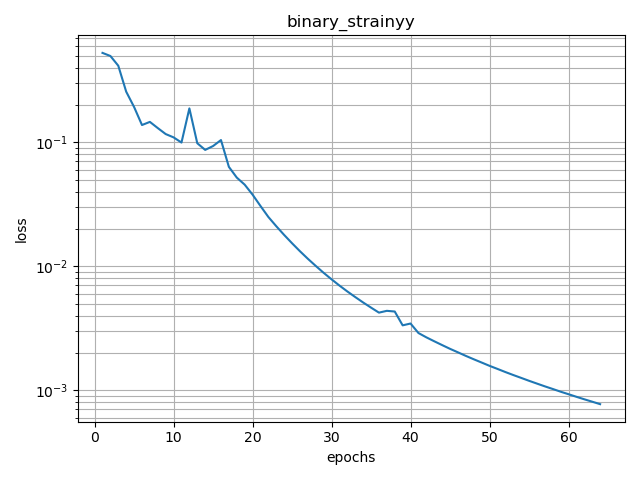
\includegraphics[totalheight=4cm]{Figures/Appendix/eyy/binary_strainyy_plot_loss.png}
    \caption{True}
  \end{subfigure}
  %
   \begin{subfigure}[b]{0.45\linewidth}
    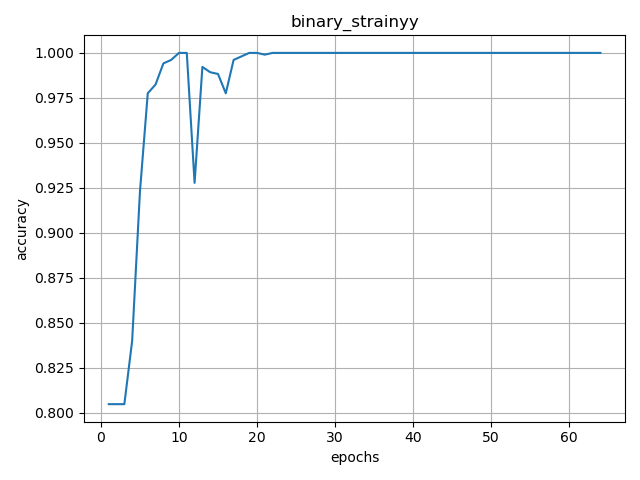
\includegraphics[totalheight=4cm]{Figures/Appendix/eyy/binary_strainyy_plot_accuracy.png}
    \caption{Training accuracy vs epochs}
   \end{subfigure}
   %
   \begin{subfigure}[b]{0.45\linewidth}
    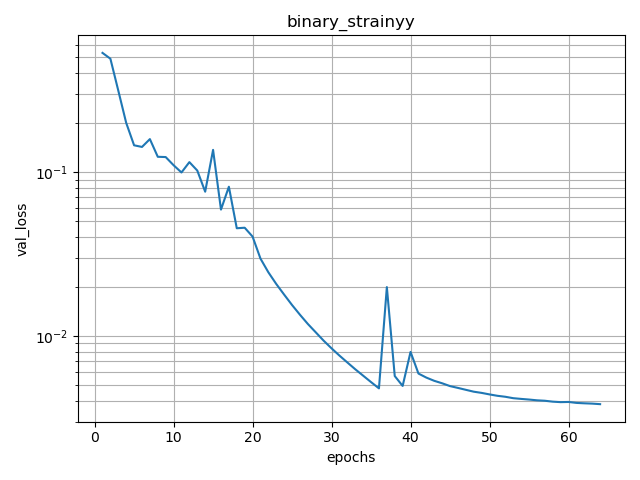
\includegraphics[totalheight=4cm]{Figures/Appendix/eyy/binary_strainyy_plot_val_loss.png}
    \caption{Validation loss function vs epochs}
   \end{subfigure}
   %
   \begin{subfigure}[b]{0.45\linewidth}
     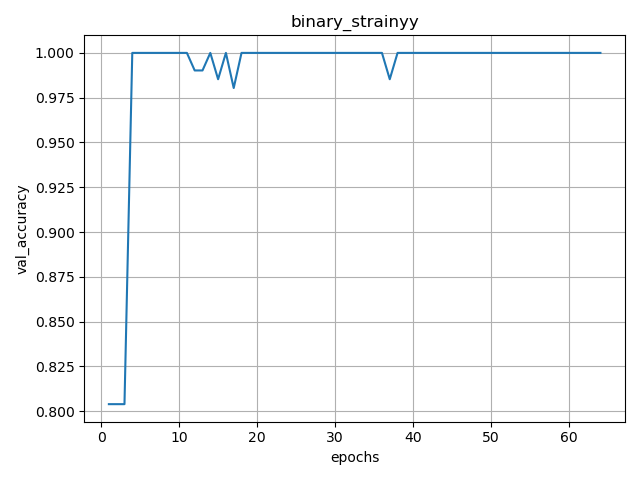
\includegraphics[totalheight=4cm]{Figures/Appendix/eyy/binary_strainyy_plot_val_accuracy.png}
     \caption{Validation accuracy vs epochs}
   \end{subfigure}
   %
  \caption{\label{app:eyy:curves} Optmization history during the training phase for binary classification using $\epsilon_{yy}$ only.}
 \end{figure}
% loss and val_loss Curves
\subsection{Case 2: Using $\epsilon_{yy}$ with noise}
\subsection{Case 3: Using $u_y$ with no noise}
% loss and val_loss Curves
\subsection{Case 4: Using $u_y$ with noise}
%

